\chapter{Lecture 14 Curve Fitting with Non-linear Functions}
\label{ch:lec14n}
\section{Objectives}
The objectives of this lecture are to:
\begin{itemize}
\item Explain how to carry out least squares curve fitting with a nonlinear equation.
\item Do an example using MATLAB.
\end{itemize}
\setcounter{lstannotation}{0}

\section{Curve Fitting with Nonlinear Equation}
The method of least squares requires the estimator to be a linear combination of functions---although, in most cases the individual functions are not linear. If the estimator is non-linear, then you need to linearize it, if possible, through an appropriate transformation.  A variety of useful transforms are presented in Table \ref{transform}.\cite[-2.5cm]{gilat}

\begin{table}[h]
\centering
\begin{tabular}{|p{0.75in}|p{1.55in}|p{1.25in}|p{1.3in}|}
\hline
Nonlinear equation & Linear Form & Relationship to $Y = a_{1}X + a_{0}$ &
Values for linear least-squares regression \\
\hline
$ y = bx^{m}$ & $\ln(y)=m\ln(x)+\ln(b)$ & $Y = \ln(y),\ \  X = \ln(x),
\ \  a_{1} = m, \ \  a_{0} = \ln(b) $ & $\ln(x_{i})$ and $\ln(y_{i})$ \\
\hline
$y = be^{mx}$ & $\ln(y)=mx+\ln(b)$ & $Y = \ln(y), X=x, a_{1}=m, a_{0} = \ln(b)$ &
$x_{i} \text{ and } \ln(y_{i})$ \\
\hline
$y = b10^{mx}$ & $\log(y) = mx + \log(b)$ & $Y = \log(y)$, $X=x$ $a_{1}=m$,
$a_{0} = \log(b)$  & $x_{i}$ and $\log(y_{i})$ \\
\hline
$y = \frac{1}{mx + b}$ & $\frac{1}{y} = mx + b$ & $Y=\frac{1}{y}$, $X=x$,
$a_{1}=m$, $a_{0} = b$ & $x_{i}$ and $\sfrac{1}{y_{i}}$ \\
\hline
$y = \frac{mx}{b + x}$ & $\frac{1}{y} = \frac{b}{m}\frac{1}{x} + \frac{1}{m} $
& $Y=\frac{1}{y}$, $X=\frac{1}{x}$, $a_{1}=\frac{b}{m}$, $a_{0}=\frac{1}{m}$ &
$\sfrac{1}{x_{i}}$ and $\frac{1}{y_{i}}$ \\
\hline
\end{tabular}
\caption[][-1.0cm]{Transforming nonlinear equations to linear form.}
\label{transform}
\end{table}
We will use these transformations in the examples that follow.

\vspace{3.5cm}

\noindent \textbf{Example \#1:} Data are provided in the table below.
\begin{table}
\begin{tabular}{|l|l|l|l|l|l|}
\hline
$x$ & 1 & 2 & 3 & 5 & 8 \\ \hline
$y$ & 0.8 & 1.9 & 2.2 & 3 & 3.5 \\ \hline 
\end{tabular}
\caption{Table of data for Example \#1.}
\label{tab:lec14n-ex1}
\end{table}

\vspace{0.2cm}

\noindent Determine the coefficients $m$ and $b$ in the function $y=\left[m\sqrt{x} + b\right]^{\sfrac{1}{2}}$ that best fits the data.  

\vspace{0.2cm}


\noindent \textbf{Solution: }Here, right off the bat, we have a case that is not represented in Table \ref{transform}.  Nonetheless, we will persevere and notice without too much difficulty that if I make the transformation $p = y^2$, then the estimator for $p$ is given by: $p = m\sqrt{x} + b$.  MATLAB code to load the data and calculate the coefficients of the, now, linearized, estimator is provided below.
\marginnote[1.5cm]{\textbf{Note: } Both of the vectors for $x$ and $y$ are constructed so as to be \emph{column vectors}.  We follow this practice for the other examples as well so that we can employ the same MATLAB equations for carrying out least squares regression and satisfy the semantics of each linear algebraic operation.}
\begin{lstlisting}[style=myMatlab]
clear
clc
close 'all'

% data
x = [1 2 3 5 8]';
y = [0.5 1.9 2.2 3 3.5]';

% linearized estimator
p = y.^2;
X = [x.^0 x.^(0.5)];

C = (X'*X)\(X'*p);

%remember to "undo" the linearizing transformation
est1 = @(x) sqrt(C(1) + C(2)*sqrt(x));
\end{lstlisting}
Notice how we needed to apply the inverse of the linearizing transformation to recover the desired estimator.  Results are shown in Figure \ref{fig:lec14n-ex1}.
\begin{marginfigure}[-4cm]
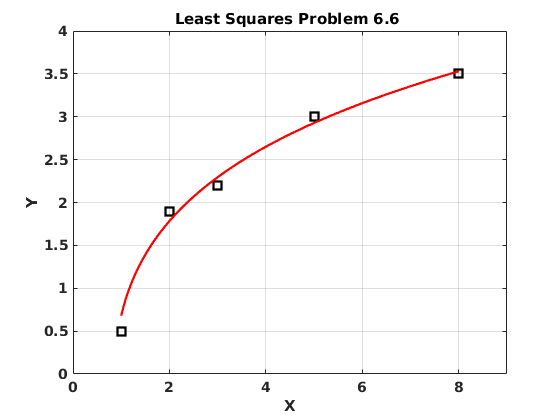
\includegraphics{lec14n-ex1.png}
\caption{Plot of least squares estimator for Example \#1.}
\label{fig:lec14n-ex1}
\end{marginfigure}

\vspace{0.5cm}

\noindent \textbf{Example \#2:} Consider the following given data.

\begin{table}
\begin{tabular}{|l|l|l|l|l|l|}
\hline
$x$ & -2 & -1 & 0 & 1 & 2 \\ \hline
$y$ & 1.5 & 3.2 & 4.5 & 3.4 & 2 \\ \hline 
\end{tabular}
\caption{Table of data for Example \#2.}
\label{tab:lec14n-ex2}
\end{table}

\vspace{0.2cm}

\noindent Determine the coefficients $a$ and $b$ in the function $y=\frac{a}{x^2 + b}$ that best fit the data.

\vspace{0.2cm}


\noindent \textbf{Solution: } The form of this non-linear estimator is similar to that presented in the 4\textsuperscript{th} row of Table \ref{transform}.  
\begin{align*}
p &= \frac{1}{y} \\
&= \frac{x^2 + b}{a} \\
&= \frac{x^2}{a} + \frac{b}{a} \\
&= c_1 x^2 + c_2
\end{align*}
where $c_1 = \sfrac{1}{a}$ and $c_2 = \sfrac{b}{a}$.  We implement the linear least squares in MATLAB in the, by now, familiar style: \marginnote[3.0cm]{

\noindent \ref{lst:ann14n-1} Since $c_1 = \sfrac{1}{a}$, then $a = \sfrac{1}{c_1}$.

\vspace{0.15cm}

\noindent \ref{lst:ann14n-1} Here $c_2 = \frac{b}{a}$ so 
\begin{align*}
c_2 a &= \frac{b}{a} a \\
&= b
\end{align*}
}
\begin{lstlisting}[style=myMatlab]
clear
clc
close 'all'

% data
x = [-2 -1 0 1 2]';
y = [1.5 3.2 4.5 3.4 2]';

% linearized estimator
X = [x.^2 x.^0];
b = y.^(-1);

C = (X'*X)\(X'*b);

% remember to "undo" the linearizing transformation
a = 1./C(1); /*!\annotation{lst:ann14n-1}!*/
b = C(2)*a;  /*!\annotation{lst:ann14n-2}!*/
\end{lstlisting}
A plot of the resulting estimator is shown in Figure \ref{fig:lec14n-ex2}.
\begin{marginfigure}[-0.25cm]
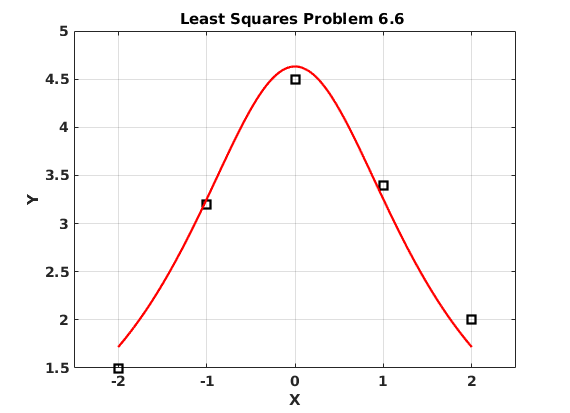
\includegraphics{lec14n-ex2.png}
\caption{Plot of least squares estimator for Example \#2.}
\label{fig:lec14n-ex2}
\end{marginfigure}

\vspace{0.5cm}

\noindent \textbf{Example \#3:} Water solubility in jet fuel, $W_s$, is a function of temperature, $T$, and can be modeled by an exponential function of the form:
\begin{equation*}
W_s = be^{mT}
\end{equation*}
Table \ref{tab:lec14n-ex3} presents measured values of water solubility over a range of temperatures.  
\begin{table}
\begin{tabular}{|l|l|l|l|l|l|}
\hline
$T \ (^{\circ}C)$ & -40 & -20 & 0 & 20 & 40\\ \hline
$W_s \ (\% wt. )$ & 0.0012 & 0.002 & 0.0032 & 0.006 & 0.0118 \\ \hline 
\end{tabular}
\caption{Table of data for Example \#3.}
\label{tab:lec14n-ex3}
\end{table}

\vspace{0.1cm}

\noindent Using linear least squares, determine the constants $m$ and $b$ that best fit the data.

\vspace{0.2cm}


\noindent \textbf{Solution: }The form of this non-linear estimator is similar to that presented in the 2\textsuperscript{nd} row of Table \ref{transform}.  To linearize the estimator we first take the natural logarithm of both sides:
\begin{align*}
\ln{W_s} &= \ln{be^{mT}} \\
\ln{W_s} &= \ln{b} + \ln{e^{mT}} \\
&= \ln{b} +  mT \\
&= c_1 T^{0} + c_2T^{1}
\end{align*}
where $c_1 = \ln{b}$ and $c_2 = m$.  We carry out the linear least squares process as usual.

\begin{lstlisting}[style=myMatlab]
clear
clc
close 'all'

% data
T = [-40 -20 0 20 40]';
W = [0.0012 0.002 0.0032 0.006 0.0118]';

X = [T.^0 T.^1];
p = log(W);

C = (X'*X)\(X'*p);

b = exp(C(1));  /*!\annotation{lst:ann14n-3}!*/
m = C(2);

est3 = @(x) b*exp(m*x);
\end{lstlisting}
\marginnote[-2.0cm]{

\noindent \ref{lst:ann14n-3} Since $c_1 = \ln{b}$ we undo the transformation by exponentiating both sides.

}

\vspace{0.1cm}

\noindent The resulting estimator is plotted against the given data in Figure \ref{fig:lec14n-ex3}.

\begin{marginfigure}
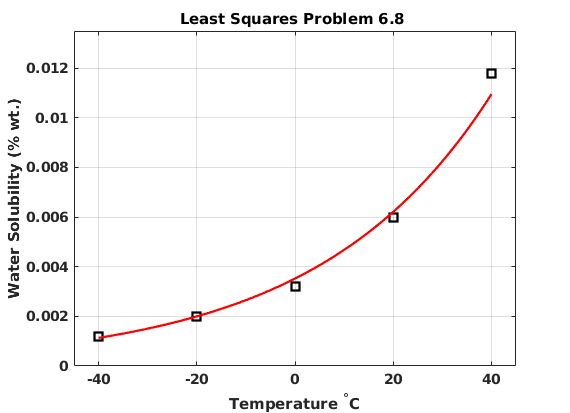
\includegraphics{lec14n-ex3.png}
\caption{Plot of least squares estimator for Example \#3.}
\label{fig:lec14n-ex3}
\end{marginfigure}




